\chapter{Electronic excitations}

We call \textit{electronic} excitations those that, at $\lambda_{ir}=0$, arise from $H_{el}$ in (\ref{eq:full-hamiltonian}). This part of the hamiltonian

\begin{equation}\label{eq:Hel} H_{el} = \sum_n \epsilon_n \rho_n + \sum_{ \langle nm \rangle \sigma } t (c_{n \sigma }^\dagger c_{m \sigma } + H.c.) + U\sum_n \rho_{n\downarrow}\rho_{n\uparrow} \end{equation}

can be represented  as a 9x9 matrix:

\begin{equation}\label{eq:Hel-matrix} \left( \begin{array}{ccccccccc} 
U+2\epsilon &\;\;t\;\;&\;\;0\;\;&\;\;t\;\;&0&\;\;0\;\;&\;\;0\;\;&\;\;0\;\;&0 \\
t&0&t&0&t&0&0&0&0 \\
0&t&2\epsilon &0&0&t&0&0&0 \\
t&0&0&0&t&0&t&0&0 \\
0&t&0&t&U-2\epsilon &t&0&t&0 \\
0&0&t&0&t&0&0&0&t \\
0&0&0&t&0&0&2\epsilon &t&0 \\
0&0&0&0&t&0&t&0&t \\
0&0&0&0&0&t&0&t&U+2\epsilon  \end{array} \right)\end{equation}

and easily diagonalized to see that its first excited state has an energy of ~1376 cm$^{-1}$ above the  ground state.


\section{Projection into definite electronic occupation states}

Since we are using basis states with definite electron occupancy, from the eigenvectors of the (\ref{eq:Hel-matrix}) matrix we can directly see the projections into definite electronic occupation states. The following table summarizes those values omitting equivalent basis states:

\begin{tabular}{| c | c | c | c | c | c | c | c | c | c |}
\hline
Energy from ground state (cm$^{-1}$) & 0.0 & 1376.42 & 3825.49 & 4325.12 & 14897.84 & 15329.82 & 53933.30 & 69272.75 & 69309.3 \\
\hline
$\uparrow \downarrow \ - \ -$ & 0.00276 & 0.00000 & 0.00382 & 0.00000 & 0.00090 & 0.00000 & 0.00179 & 0.49618 & 0.49455 \\
$\uparrow\  \downarrow \ -$ & 0.20130 & 0.19717 & 0.24809 & 0.25000 & 0.04045 & 0.05283 & 0.00606 & 0.00191 & 0.00219 \\
$\uparrow \ - \ \downarrow$ & 0.08522 & 0.10566 & 0.00000 & 0.00000 & 0.41451 & 0.39434 & 0.00023 & 0.00000 & 0.00000 \\
$ - \ \uparrow \downarrow \ -$ & 0.01884 & 0.00000 & 0.00000 & 0.00000 & 0.00736 & 0.00000 & 0.97174 & 0.00000 & 0.00205 \\
\hline
\end{tabular}

We noticed\cite{GarciaSaraviaOrtizdeMontellano2013} that, for the first \textit{electronic} excitation, the projection into states with an electron in each oxygen decreases with an increasing $\lambda_{ir}$ suggesting partial charge localization.

\section{Projection into phonon coordinates}

\begin{figure}[ht!]
\centering
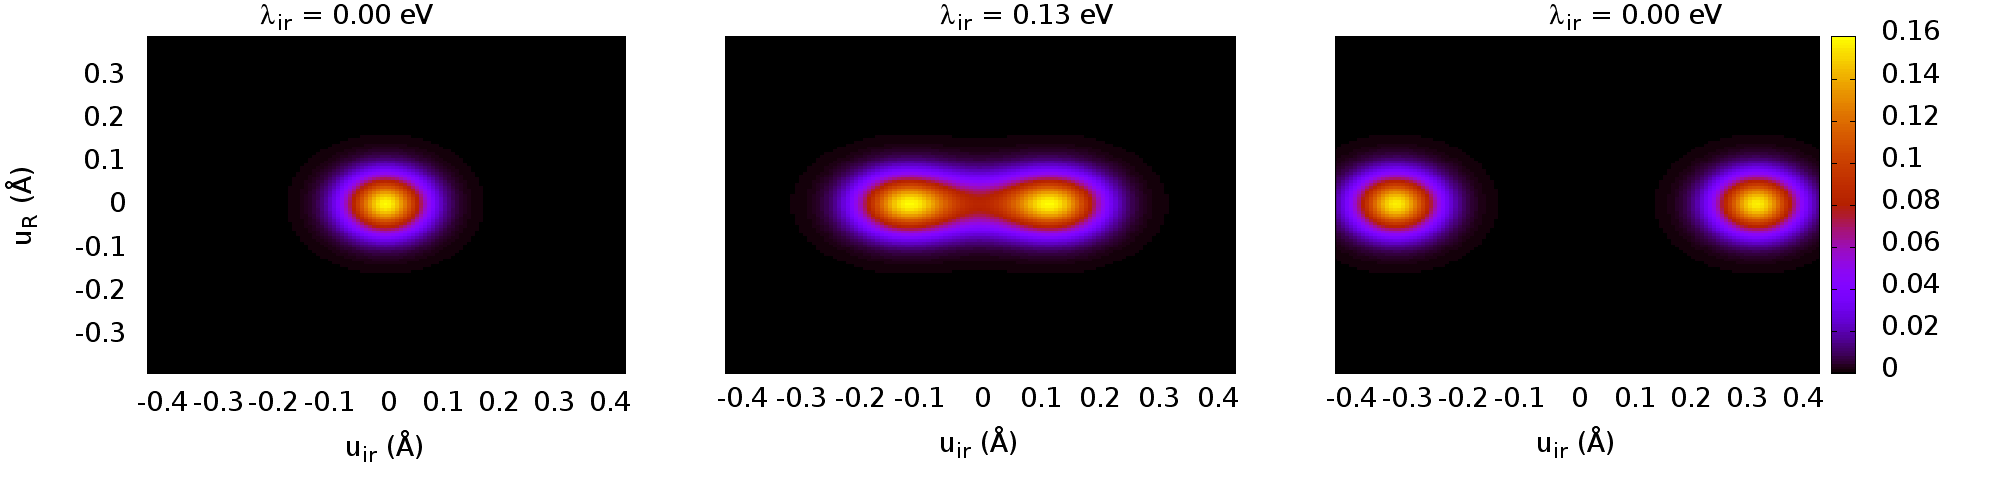
\includegraphics[width=0.8\textwidth]{images/ph-electronic.png}
\caption{Electronic state projected into phonon coordinates for three representative electron-lattice coupling ($\lambda_{ir}$) values.}
\label{fig:ph-electronic.png}
\end{figure}


\section{Projection onto itself at zero electron-lattice coupling}


To find more information about the nature of this \textit{electronic} state we performed a projection of it's eigenvector when $\lambda_{ir}=0$ with its eigenvector when $0<\lambda_{ir}\leq 0.25\ eV$. This should give us a sense about how much this state changes due to the electron-lattice coupling. The next figure is a plot of this projection. 

\begin{figure}[ht!]
\centering
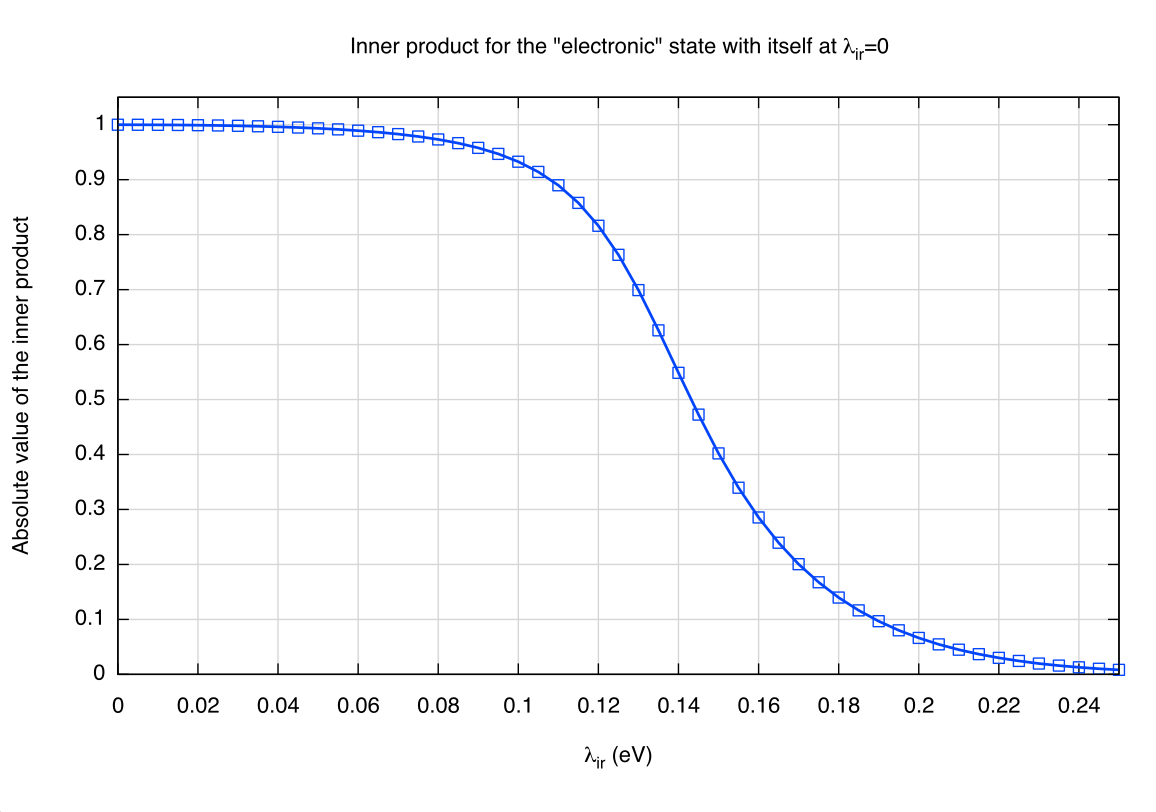
\includegraphics[width=0.8\textwidth]{images/electonic-state-inner-product.png}
\caption{Inner product of the electronic state with itself at $\lambda_{ir}=0$.}
\label{fig:electonic-state-inner-product}
\end{figure}

As expected this product is close to 1 for small $\lambda_{ir}$. It starts to differ significantly for $\lambda_{ir}\sim0.1$ eV having the strongest change at around $\lambda_{ir}\sim0.14$ eV and asymptotically approaching zero afterwards.

\section{Isotopic shift}

\begin{figure}[ht!]
\centering
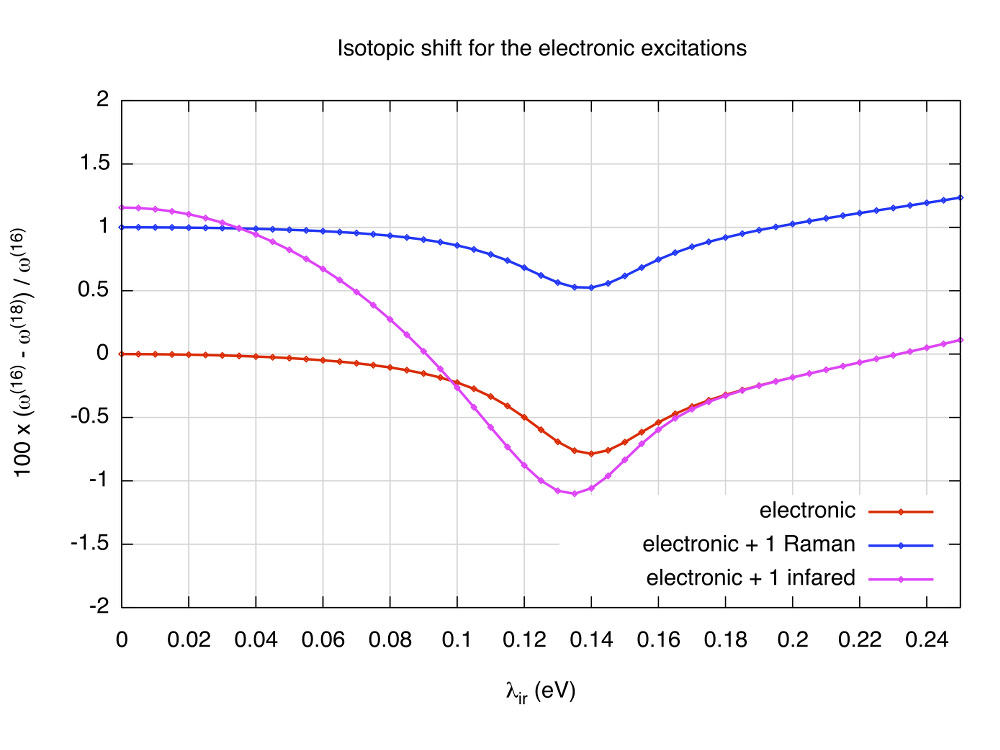
\includegraphics[width=0.8\textwidth]{images/isot-el.jpg}
\caption{Isotopic shift for the electronic state.}
\label{fig:isot-el}
\end{figure}

